% !TEX encoding = UTF-8 Unicode
\documentclass[a4paper]{article}


\usepackage[T1]{fontenc}     % För svenska bokstäver
\usepackage[utf8]{inputenc}  % Teckenkodning UTF8
\usepackage[swedish]{babel}  % För svensk avstavning och svenska
                             % rubriker (t ex "Innehållsförteckning")
\usepackage{fancyvrb}        % För programlistor med tabulatorer
\fvset{tabsize=4}            % Tabulatorpositioner
\fvset{fontsize=\small}      % Lagom storlek för programlistor

\title{TurtleRace \\
	Inlämningsuppgift 1, Programmeringsteknik för C/D}
\author{Bernt Christensen, C11 (dic11bch@student.lu.se)\\
Johan Bäversjö, C11 (dic11jba@student.lu.se)}


% *** Tillägg för denna rapport. ***
% Paket:
\usepackage{graphicx}         % För att inkludera bilder.

% Kommandon i denna rapport
\newcommand{\code}[1]{\texttt{#1}} % För programkod i text.
% *** Slut på tillägg för denna rapport. ***


\begin{document}              % Början på dokumentet

\maketitle
\thispagestyle{empty}
\newpage
\setcounter{page}{1}
\section{Bakgrund}
Uppgiften består i att skapa en tävlingsbana som är oberoende av vad för tävling som utförs på den, en tävling där två stycken sköldpaddor tävlar mot varandra samt att genomföra själva loppet där dessa två sköldpaddor möts.

Så här kommer ett lopp att se ut:
\begin{center}
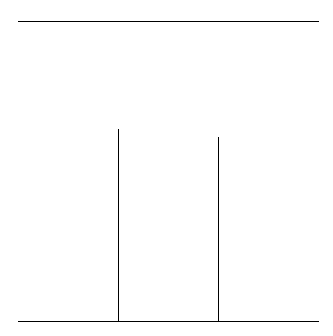
\includegraphics[scale=0.29]{turtle_race.png}
\end{center}
Längst ner och högst upp på bilden kan start- respektive mållinje ses. De två lodräta linjerna representerar de sköldpaddor som tävlar mot varandra.

Fokus i uppgiften ligger på hur programmet skall utformas snarare än vad som utförs. 

\section{Modell}
Modellen av loppet innehåller följande klasser:


\begin{tabular}{lp{8cm}}
\code{TurtleRace} & Innehåller \code{main}-metoden som initierar alla objekt som behövs för att genomföra ett lopp. \\
\code{Turtle} & Klass som beskriver en Turtle i planet. \\
\code{RaceTrack} & Klass som beskriver en banas utseende, är oberoende av vilken typ av objekt som tävlar. \\
\code{RacingEvent} & Beskriver en tävling. Håller reda på bana samt deltagare \\

\end{tabular}

\vspace{\baselineskip}
Loppet implementeras genom att programmet itererar tills en av sköldpaddorna nått mållinjen.
Nedan följer en beskrivning till flödet i programmet:

\begin{itemize}
\item Fönstret, banan och sköldpaddorna initieras. Banan ritas ut i fönstret av typ \code{SimpleWindow} i klassen \code{RaceTrack}.
\item Ett lopp skapas med klassen \code{RacingEvent}
\item Loppet initieras i och med ett musklick i fönstret. Då ställs sköldpaddorna först upp på startpositionerna, som hämtas från \code{RaceTrack},  i metoden \code{race()} från klassen \code{RacingEvent}
\item Metoden \code{race()} returnerar när en av sköldpaddorna nått mållinjen, därefter är programmet färdigt. 
\end{itemize}

\section{Brister och kommentarer}
Programmet kan endast hantera ett lopp mellan två stycken sköldpaddor i dess nuvarande utförande. För att kunna lägga till sköldpaddor behövs stora redigeringar i koden göras.

En förbättring hade varit att använda en vektor istället för dynamiskt kunna bestämma antalet skäldpaddor.

Båda sköldpaddorna har okända namn, vilket medför att det inte är möjligt att ta reda på vilken sköldpadda som vunnit bortsett från det visuella resultatet. 

För att kunna koppla ihop det här programmet med andra system hade vi till exempel låtit användaren specifiera alla sköldpaddor som parametrar för programmet vid uppstart. Programmet hade sedan skrivit ut namnet på vinnaren.


\section{Programlistor}
Klasserna finns i filer med motsvarande namn. Till exempel innehåller filen  \code{RaceTrack.java} klassen \code{RaceTrack}. Alla klasser som används finns i samma katalog som huvudprogrammet

\subsection{\code{TurtleRace}}
\VerbatimInput{../src/TurtleRace.java}


\subsection{\code{Turtle}}
\VerbatimInput{../src/Turtle.java}

\subsection{\code{RaceTrack}}
\VerbatimInput{../src/RaceTrack.java}

\subsection{\code{RacingEvent}}
\VerbatimInput{../src/RacingEvent.java}


\end{document}                  % Slut på dokumentet
